% !TEX root = ThesisGchatzi.tex

\section{Experimental Evaluation}
\label{sec:knn_experiment}

\graphicspath{{Papers/SpringerJournalOfBigData/}}

FML-$k$NN was assessed in terms of wall-clock completion time and scalability, by conducting a comparative benchmarking among similar implementations, executed over different distributed processing engines. The latter are either executed in one (where possible), or three Spark or Hadoop (i.e., an extension of the original H-z$k$NNJ algorithm) sessions and are compared with the corresponding versions of the probabilistic classifier. Similar results are expected for the regressor which we have omitted to avoid repetition.

We also present two case studies which exhibit the framework's efficiency over useful insights extraction from water consumption events on a city scale level. Throughout our experiments, we used one synthetic and two real-world water consumption time-series datasets.

\subsection{Experimental setup}
\label{subsec:expsetup}
In the following, we present the environmental setting of the experiments and the qualitative and quantitative metrics that we used to assess the performance of the classification and regression processes. We also present the parameters that were used and how they were determined in the context of the experimentation process.

\paragraph{System}
\label{par:system}
The algorithms were assessed on a pseudo-distributed environment. The setup includes a system with 4 CPUs, each containing 8 cores clocked at 2.13GHz, 256 GB RAM and a total storage space of 900 GB. The CPUs support hyper-threading technology, running 2 separate threads per core. The total parallel capability of the system reaches the 64 threads ($4 \cdot 8 \cdot 2$). All (i.e., Flink-, Spark- and Hadoop-based) implementations were evaluated on the same HDFS, over a local \textit{YARN} (Yet Another Resource Negotiator) resource manager. This way, each Flink task manager, Spark executor or Hadoop daemon runs on a different YARN container, represented by a separate Java process able to run one or more threads, simulating the distributed cluster.

Despite the significant differences in the distributed processing engines' configuration settings, they were all configured in order to use the same amount of system resources. The level of parallelism of all tasks for each engine was set to 16, in order to exploit the fact that, in an optimally determined setting and during the experiments, the stage 2 partitions the dataset into 8 subsets and the total number of shifts is 2. Thus, a maximum of 16 simultaneous tasks are executed in all cases. For Flink and Spark, a total of 4 task managers (one per CPU) and executors respectively were assigned 32768 MB of Java Virtual Machine (JVM) heap memory. Each task manager and executor was given a total of 4 processing slots (Flink) or executor cores (Spark). For Hadoop, the parallelism ability was set to 16 by assigning the mappers and the reducers to the same number of YARN containers, with 8192 MB of JVM each. Thus, the total amount of JVM heap memory assigned to each session is always 131072 MB (either $4 \cdot 32768$ MB, or $16 \cdot 8192$ MB).

Despite our attempt to assign similar amount of system resources to each distributed processing engine and due to the fact that each one offers a handful of configuration settings regarding execution, memory allocation, and job scheduling behavior, the performance of the different implementations may differ from the optimal one. However, after performing numerous benchmarking sessions, we believe that for the current system setting, the presented configuration is fair, achieving the highest possible performance for all three engines, while maintaining the level of parallelism at 16. The configuration was performed by taking into consideration the corresponding guide of each engine.

\paragraph{Parameters}
\label{par:Parameters}
FML-$k$NN uses a variety of input parameters required by the underlying distributed $k$NN algorithm, in order to support the classification and regression processes. Regarding the value of the $k$ parameter that was used throughout the experiments and due to the fact that the optimal value is problem specific, we performed a separate \textit{cross-validation}-based evaluation for each of the case studies (see Section~\ref{subsec:case_studies}). The best $k$ parameter choice was performed in a way that maintains the best balance between completion time and accuracy. Most parameters were similarly chosen after performing appropriate cross-validation-based benchmarking.

Among the rest of the parameters, FML-$k$NN utilizes a vector of size equal to the input dataset's dimensions, indicating the weight of each feature according to its significance to the problem. Each feature is multiplied with its corresponding weight before the execution of the algorithm in order to perform the required scaling, according to the feature's importance. To automatically determine an optimal feature weighting vector, we provide the option of executing a genetic algorithm, which uses a specific metric, described in the next paragraph, as cost function. The parameters of the genetic algorithm, such as the size of the \textit{population}, the probability to perform \textit{mutation} or \textit{crossover}, the \textit{elite} percentage of the population and the number of the iterations can be directly determined by the user. This approach was applied to produce the optimal feature weighting vector for each of the cases that we studied.

\paragraph{Metrics}
\label{par:metrics}
Four different well known performance measures were used to evaluate the quality of the results obtained by the classifier and the regressor. These performance measures are included in the framework in order to offer the ability to assess the various data analysis tasks. \textit{Accuracy} and \textit{F-Measure} are implemented for classification, while \textit{Root Mean Square Error} (RMSE) and \textit{Coefficient of determination} ($R^2$) are used to evaluate the quality of regression. A short description of what each of these metrics represents in our experimentation is listed below:

\begin{itemize}
\item \textbf{Accuracy}: The percentage of correct classifications (values from 0 to 100). It indicates the classifier's ability to correctly guess the proper class for each element.
\item \textbf{F-Measure}: The weighted average of \textit{precision} and \textit{recall} of classifications (values from 0 to 1). Using this metric, we ensure good balance between precision and recall, thus, avoiding misinterpretation of the accuracy.
\item \textbf{Root Mean Square Error (RMSE)}: Standard deviation between the real and predicted values via regression. This metric has the same unit as the target variable. It provides us with the insight of how close the guessed values are to the real ones.
\item \textbf{Coefficient of determination ($R^2$)}: Indicates the quality of the way the model fits the input data. It takes values from 0 to 1, with 1 being the perfect fit. A good fit means that the regressor is able to properly identify the variations of the training data.
\end{itemize}

The completion time comparison of the distributed processing engines is performed after simply obtaining the system time elapsed before and after each execution.

\subsection{Datasets}
\label{subsec:datasets}
For the experimental evaluation of FML-$k$NN we used two real-world water consumption related datasets coming from Switzerland and Spain. We also generated a synthetic dataset, based on an extended version of the Spain dataset, with a much larger amount of entries. Since the framework's algorithm is $k$NN-based, we normalized all the datasets' features from values ranging from 0 to 1, in order to avoid broader ranged features heavily affecting the result. 

\paragraph{SWM dataset}
\label{par:alicante}
As in the previous chapters, this dataset is a courtesy of the DAIAD project (\url{http://daiad.eu/}). Specifically, it contains hourly time-series of 1000 Spanish households' water consumption, measured with smart water meters. It covers a time interval of a whole year, i.e., from the 1$^{st}$ of July 2013 to the 30$^{th}$ of June 2014. The records include a household identifier, a timestamp and a meter measurement in liters. This dataset has a total number of 8.7M records.

\paragraph{Shower dataset}
\label{par:amphiro}
The second dataset is also provided by DAIAD and includes shower events from 77 Swiss households collected with shower water meters. Each record contains a household and shower identifier, a meter measurement in liters, the number of times that the faucet was turned off during the shower and the corresponding duration, the total duration of each shower as a whole, as well as the average water temperature and flow rate. It also contains demographic information related to the age, income, number of males or females and total number of household members. This dataset counts 5795 records. While this dataset is not on a Big Data scale, we perform a case study based on it, in order to assess the framework's data analysis capability on water consumption data regarding a single water fixture and consumer activity.

\paragraph{Synthetic dataset}
\label{par:synthetic}
In order to evaluate completion time performance on Big Data, we created a synthetic dataset via a Big Data generator. The latter is a part of the \textit{BigDataBench} benchmark suite~\cite{bdbench} and operates via .xml files, in which the user can determine the number of records and their features. Based on an extended version of the SWM dataset produced after proper feature extraction (see Section~\ref{par:feat_extr1}), the synthetic dataset's entries consist of an id, 10 features and two target variables of continuous (floating point with 10 decimals) and binary data representation, respectively. Each feature is ranged from 1 to 99 and the id is alphanumeric. The data representation, number and range of features was selected in order to maintain a relatively high number of dimensions, while being able to create a large number of records and at the same time avoiding exceeding the memory limits of the setup (approx. 8192 MB per mapper or reducer for the Hadoop case). Thus, the total size of the synthetic dataset has 100M records (approx. 4.1 GB).

\subsection{Benchmarking}
\label{subsec:fml$k$NN_performance}
In the following, we perform a comparative benchmarking of FML-$k$NN, in terms of scalability and wall-clock completion time, using the synthetic dataset and the probabilistic classifier. Similar results are expected for the regressor. The comparison involved:

\begin{itemize}
	\item \textbf{FML-$k$NN (single session)}: The proposed implementation, presented in the previous section.
	\item \textbf{FML-$k$NN (three sessions)}: A three-sessions version of FML-$k$NN, where each stage is executed by a different Flink process.
	\item \textbf{S-$k$NN (single session)}: An Apache Spark version with the same architecture as FML-$k$NN.
	\item \textbf{S-$k$NN (three sessions)}: A three-sessions version of S-$k$NN, where each stage is executed by a different Spark process.
	\item \textbf{F-z$k$NN}: The single-session algorithm on which the core algorithm of FML-$k$NN was based.
	\item \textbf{H-z$k$NNJ}: An extended version of the algorithm to perform probabilistic classification executed in three separate sessions. This is the baseline method. 
\end{itemize}

It is important to note that a single-session version of the H-z$k$NNJ algorithm is not possible, as a Hadoop session can only execute one map, followed by one reduce procedure. A single session requires the three stages to be executed in a sequential manner, which is not possible in Hadoop, as it would require mapping to be performed after reducing procedures several times.

\subsubsection{Wall-clock completion time}
\label{subsubsec:comp_time}
Table~\ref{table1} shows the probabilistic classifier's wall-clock completion time of all Flink, Spark and Hadoop versions, run in either three, or one sessions (possible only for FML-$k$NN, S-$k$NN and F-z$k$NN). The three-session F-z$k$NN is identical to the three-session FML-$k$NN implementation and its measurements are omitted. We used the synthetic dataset and we followed a 10\%--90\% testing--training split scheme, resulting in 10M records being used as the testing set ($R$) and 90M as the training set ($S$). It is apparent that the Flink-based implementations perform significantly better than all implementations, in both three and single-session versions. This improved performance is due to Flink's ability to process tasks in a pipelined manner, which allows the concurrent execution of successive tasks, thus, gaining in performance by compensating time spent in other operations (i.e., communication between the cluster's nodes). 

The unified version implemented with Spark is significantly faster than the total wall-clock time of the corresponding three-sessions setting. This is due to the reduction of the I/O operations on HDFS during the beginning and end of each session. A critical role is also played by the omission of the mappers of stage 3, which introduced the additional overhead of forwarding the results of the second session to the proper reducers. For FML-$k$NN, the total time of the three-sessions version is similar to the unified one, again due to the pipelined way of execution, which compensates the time lost during HDFS I/O operations. The wall-clock completion time of S-$k$NN is only slightly lower for each stage than the baseline H-z$k$NNJ implementation, except during the third session, where it executes almost twice as fast. This is caused by the fact that the stage 3 does not include costly operations such as sorting and transforming the dataset coming from stage 2. The latter is partitioned according to the id of each query element (i.e., elements in $R$ dataset), thus, taking advantage of all system resources and possibly Spark's documented better performance over Hadoop. F-z$k$NN performs worse than the rest of the implementations due to its resource-hungry propagation of the transformed dataset during the first stage.

\begin{table}[!ht]
\centering
\caption{Wall-clock completion time}
\label{table1}
\begin{tabular}{l|c|c|c|c||c}
\multicolumn{1}{c|}{\multirow{2}{*}{Version}} & \multicolumn{4}{c||}{3 Sessions}             & 1 Session  \\ \cline{2-6} 
\multicolumn{1}{c|}{}                         & 1st      & 2nd      & 3rd      & Total    & Total    \\ \hline
FML-$k$NN                                         & 03m 45sec & 24m 59sec & 01m 48sec & 30m 32sec & 30m 25sec \\ \hline
S-$k$NN                                         & 07m 12sec & 29m 15sec & 03m 01sec & 39m 28sec & 33m 03sec \\ \hline
F-z$k$NN                                         & N/A & N/A & N/A & N/A & 46m 09sec \\ \hline
H-z$k$NNJ                                       & 06m 00sec & 31m 19sec & 05m 54sec & 43m 13sec & N/A     
\end{tabular}
\end{table}

It should be noted that the results do not suggest that Flink is superior to the other distributed processing engines. The comparison is limited to the current FML-$k$NN's core algorithm and the implementation and experimental setting are as fair as possible, considering the engines' different operational support. It proves, however, that our algorithm performs significantly better with Flink and supports our choice to use it as an underlying execution environment.

\subsubsection{Scalability}
\label{subsubsec:scalability}
The various implementations were also evaluated in terms of scalability. Figure~\ref{figure6} shows the way each version scales in terms of completion time for subsets of the synthetic dataset of different size, using the same 10\%--90\% testing--training split scheme. The subset sizes varied from 10M (1M testing--9M training), to 100M (10M testing--90M training). As illustrated in the figure, the FML-$k$NN implementations exhibit similar performance and scale better as the dataset's size increases. However, the unified version, i.e., the one used at FML-$k$NN framework, has the advantage of not requiring user input and session initialization between the algorithm's stages. Flink's pipelined execution advantages are once again apparent if we compare the scalability performance of all the three-sessions implementations: The I/O HDFS operations cause the Spark and Hadoop versions to scale significantly worse than Flink, which performs similarly to the unified version. Finally, due to the aforementioned dataset propagation, F-z$k$NN scales worse than all the implementations.

\begin{figure}[!ht]
	\centering
	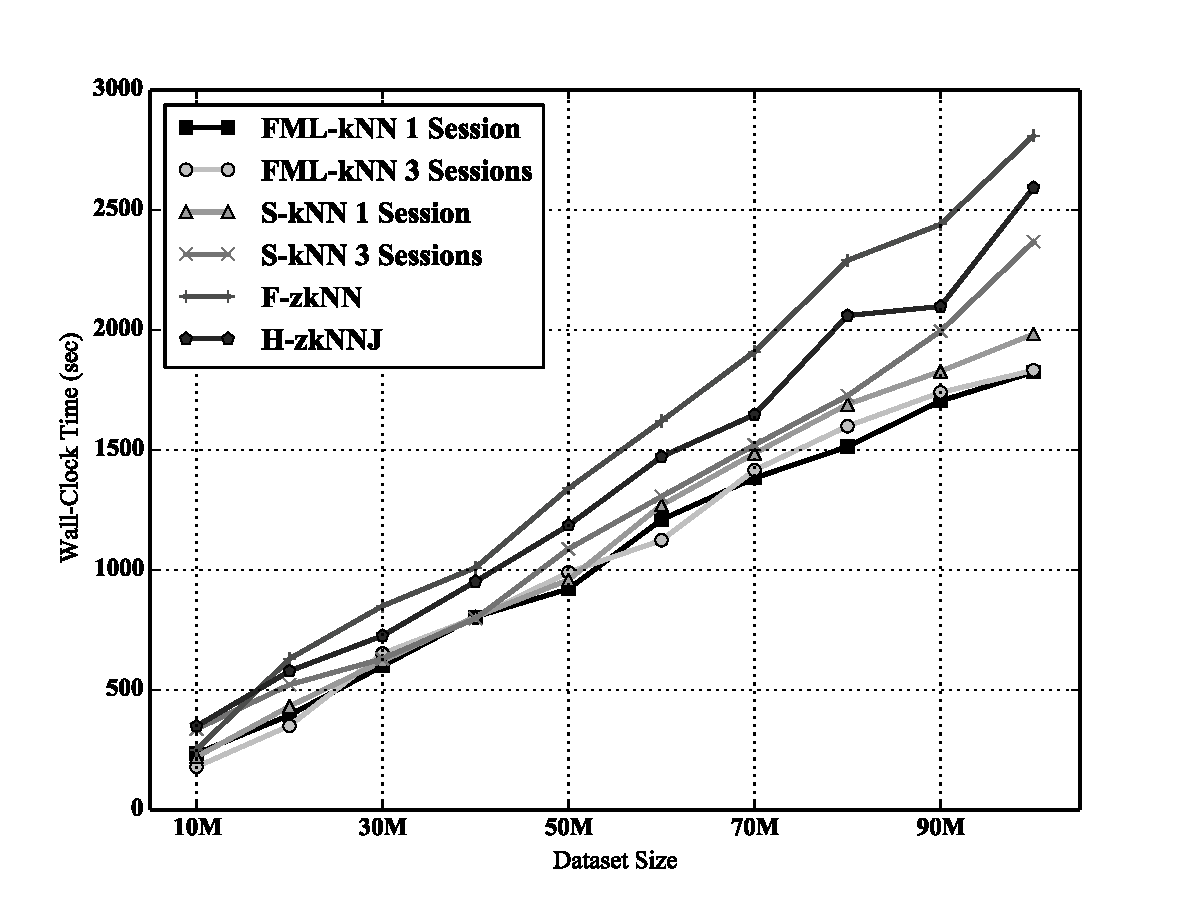
\includegraphics[width=0.65\textwidth]{figures/figure6.pdf}
	\caption{Scalability comparison for 10\%--90\% split.}
	\label{figure6}
\end{figure}

We have executed the algorithm using the 100M synthetic dataset for different split schemes, more specifically for 10\%--90\%,  30\%--70\%, 50\%--50\%, 70\%--30\% and 90\%--10\% testing--training. The results are depicted in Figure~\ref{figure7}. FML-$k$NN performs better in all cases. Due to the fact that the CPU cost of all methods similarly depends on the size of $R$ and $S$ datasets (please refer to Section~\ref{par:cost}), there are no large variations between the differences in the performance among all the implementations, and for all split cases. More time is required to finish execution as the size of the $R$ dataset is increased, due to the fact that the communication cost more heavily depends on the size of the $R$ dataset. However, this is compensated in each split case by the reduced size of dataset $S$, causing the execution time to be increased in a similar to logarithmic manner.

\begin{figure}[!ht]
	\centering
	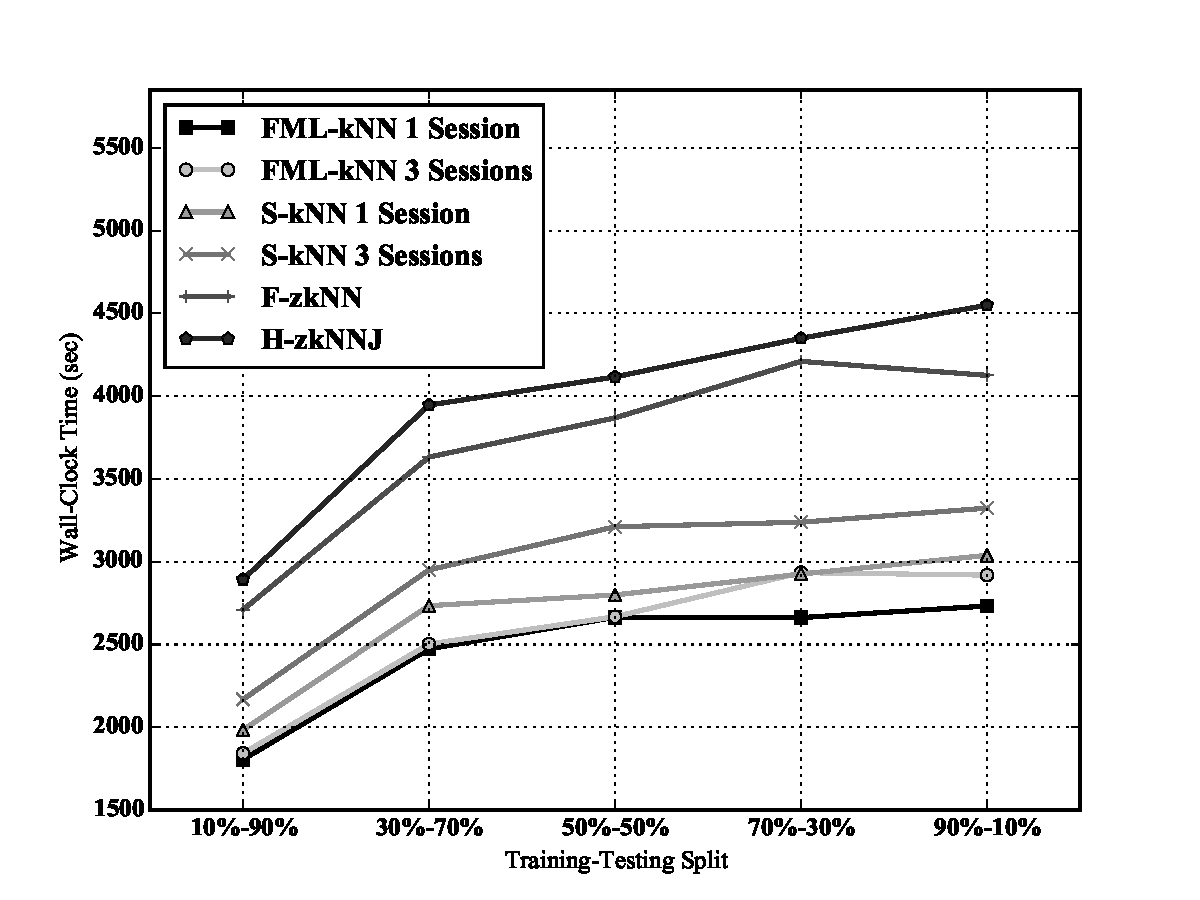
\includegraphics[width=0.75\textwidth]{figures/figure7.pdf}
	\caption{Wall-clock completion time for different split sizes.}
	\label{figure7}
\end{figure}

\subsection{Case studies}
\label{subsec:case_studies}
The framework's data analysis potential was evaluated using two real-world water related datasets in two independent case studies presented below. We focus on knowledge extraction from large volumes of historical water consumption data, towards the facilitation of useful insights acquisition for consumers and resource utilities in the water domain, which could induce lifestyle changes by promoting sustainability.

\subsubsection{SWM dataset}
\label{subsubsec:case_study1}
The first case study showcases the potential of the framework's machine learning algorithms on a water consumption time-series forecasting task. Time-series data on water consumption pose several challenges on applying machine learning algorithms for forecasting purposes. Apart from the actual measurement values, one must take into account their correlation with previous values, their seasonality, the effect of contextual factors, etc.~\cite{wrcr12805}. Thus, proper features that represent and correlate different aspects of the data need to be defined in order to take advantage of the time-series nature of such data.

\paragraph{Feature extraction}
\label{par:feat_extr1}
The dataset consists of 8.7M smart water meter hourly readings for 1000 households during a year, with each reading representing a record. The id of each element was set to be the smart meter id, together with the date and hour during which the consumption occurred. Initially, we removed any outlier records that could affect the final result. Such records belong to customers who do not exhibit normal water consumption behavior, i.e., they are frequently absent during the year or they continuously consume water (i.e. indication of possible leakage). We considered as frequently absent the users who did not consume any water for more than 40 days during a year, which indicates that they were away from their households. As a next step, we generated a total of nine different features for each data element. 

Due to the qualitative nature of the extracted features, the Euclidean distance of FML-$k$NN cannot be applied directly on them. To overcome this, we assign each feature with a new value, which is derived during a pre-processing step, after we sort according to average water consumption. For example, for the feature indicating the season of the year, we obtain the average per season water consumption and we sort the seasons according to this value. Then, each season is assigned with a numerical value corresponding to its position in this sequence. This way, if supposedly winter was assigned with 1, summer with 2, autumn with 3 and spring with 4, we know that winter is closer to summer both in terms of consumption and Euclidean distance. The extracted features are presented in more details in the following.

\begin{itemize}
\item \textbf{Hour}: The hour during which the consumption occurred.
\item \textbf{Time Zone}: We grouped the hours into four time zones of consumption: 1am - 4am (sleeping), 5am - 10am (morning activity), 11am - 7pm (working hours) and 8pm - 12am (evening activity).
\item \textbf{Day of week}: The day of the week from Monday to Sunday.
\item \textbf{Month}: The month of the year, from January to December.
\item \textbf{Season}: The season of the year, from winter to autumn.
\item \textbf{Weekend}: A binary feature indicating whether or not the consumption occurred during a weekend. We decided to include this feature after noticing differences between average hourly consumption during weekdays and weekends.
\item \textbf{Customer group}: We run a \textit{$k$-means} clustering algorithm, configured to run for time-series data, on the weekly average per-hour consumption time-series for each customer (for details, see below).
\item \textbf{Customer ranking}: For each hour, we calculated the average hourly consumption of each customer and sorted according to it.
\item \textbf{Customer class}: This feature represents a grouping of the customers to one of four classes according to their monthly average consumption, i.e. ``environmentally friendly'', ``normal'', ``spendthrift'', ``significantly spendthrift''.
\end{itemize}

Each record also contained two target variables, being the exact meter reading at each timestamp and a binary flag, indicating whether consumption occurred during that hour or not (i.e., if the meter reading was positive or zero).

The reason for choosing $k$-means for extracting the customer group feature was its significantly lower complexity compared to other clustering methods. As several evaluating works in the literature suggest \cite{singh2012performance,panda2012comparing,sehgal2014comparison}, $k$-means achieves the best performance in terms of execution time and scalability. This is crucial in our case, as in a real world scenario the feature extraction procedure, as a pre-processing step is usually required to be as time efficient as possible. Additionally, $k$-means can produce accurate and tight clusters compared to similar methods \cite{jung2014clustering}, which renders it the best choice for this case study.

Since the input data to be clustered are time-series, we used \textit{Dynamic Time Warping} (DTW) as a distance metric. DTW is a very commonly used metric for comparing time series. As opposed to other distance metrics (e.g., Euclidean distance), it can handle the case where two time series have similar form but are slightly shifted in the time axis. For more details and a formal definition of DTW, the reader can refer to~\cite{yi1998efficient}. Finally, we applied $k$-means on the average consumption time-series, with 10 as the number of clusters, which was determined as follows. Initially, we used a rule of thumb which provides a very fast estimation of the optimal number of clusters, described by Kodinariya et al.~\cite{kodinariya2013kmeans}, which calculates $k$ as follows:
\begin{equation}
	k=\sqrt[]{\frac{n}{2}}
\end{equation}
where n is the number of elements to be clustered. Considering the number of the customers (1,000), the above equation yielded $k=22$. Starting from this value, we run the $k$-means algorithm several times, using lower (higher) number of clusters than 22. We decreased (increased) the number of clusters by 1 and repeated the clustering and measured the \textit{Davies-Bouldin index}~\cite{davies1979bouldin} score of each execution. Finally, we chose the local best score, which in this case study was 10 clusters.

\paragraph{Procedure}
\label{par:procedure1}
We first execute the probabilistic classifier, with the testing set ($R$) comprising of the last two weeks of water consumption for every user (approximately 336,000 records), in order to obtain the possibility of whether consumption will occur or not, during each hour. The rest of the dataset (approximately 8.36M records) is used as the training set ($S$). We perform binary classification, obtaining an intermediate dataset indicating whether or not consumption will occur for each training record. Using the hours during which we predicted that water will be consumed, we ran the regressor, obtaining a full predicted time-series result of water consumption for each user. Before each algorithm's execution, we determined the optimal scale vector using the genetic approach.

In order to choose the optimal $k$ parameter for both algorithms, we employed a ten-fold \textit{cross-validation} approach. We iteratively split the entire dataset into ten equal parts and executed each algorithm the same number of times, using a different subset as training set ($S$) while the rest of the sets, unified, comprised the testing set ($R$). As a metric, we used accuracy for classification and RMSE for regression. The $k$ value that achieved the best balance between completion time and result quality was 15, for both the classifier and regressor.

\paragraph{Space filling curves accuracy evaluation}
\label{par:sfc_eval}
FML-$k$NN supports three SFC-based solutions for reducing the dimensionality of the input data to just one dimension, namely the $z$-order, Grey code and Hilbert curves. We evaluated the completion time and approximation quality of each SFC, in order to choose the one that achieves the best balance between timing performance and approximation accuracy, regarding the water consumption dataset. Table~\ref{table2} presents the metric and time performance related results of the probabilistic classifier and regressor for each SFC, which we obtained from running the algorithms using the ten-fold cross-validation.

\begin{table}[!ht]
\centering
\caption{Space Filling Curves' performance.}
\label{table2}
\resizebox{\columnwidth}{!}{
\begin{tabular}{c|c|c|c||c|c|c}
\multirow{2}{*}{Curve}                    & \multicolumn{3}{c||}{Classification}    & \multicolumn{3}{c}{Regression}               \\ \cline{2-7} 
                                     & Accuracy & F-Measure & Wall-Clock Time & RMSE  & R\textasciicircum 2 & Wall-Clock Time \\ \hline
\multicolumn{1}{l|}{$z$-order Curve}   & 70.24\%    & 0.775     & 1m 20sec        & 18.86 & 0.64                & 0m 59sec        \\ \hline
\multicolumn{1}{l|}{Hilbert Curve}   & 70.54\%    & 0.78      & 1m 32sec        & 18.69 & 0.66                & 1m 15sec        \\ \hline
\multicolumn{1}{l|}{Gray-code Curve} & 70.4\%     & 0.777     & 1m 25ec         & 18.81 & 0.64                & 1m 5sec        
\end{tabular}}
\end{table}

All three SFCs demonstrate similar performance in all aspects. Hilbert curve scores higher in all metrics as expected, however only slightly. Consequently, we chose the $z$-order curve for this case study, as it exhibits better time performance due to its decreased calculation complexity.

\paragraph{Results}
\label{par:res1}
The classifier correctly predicted the 74.54\% (F-Measure: 0.81) of the testing set's target variables, i.e., the hours during which some consumption occurred for the two-week period. For these specific hours the regressor achieved a RMSE score of 19.5 and a Coefficient of determination score of 0.69. The results were combined into a single file, forming the complete time-series of the dataset's last two weeks' (June 16-30 2014) water consumption prediction for all the users. 

Figure~\ref{figure8} shows four users' consumption prediction versus the actual one, during four different days. The prediction for user \#4 was close to reality. The results seem to follow the real values, but are not able to properly follow the observed ones. This indicates that it is rather difficult to accurately predict a single user's future water consumption, due to possible unforeseen or random events during a day, a fact which justifies the rather large RMSE score. For example, consumptions higher than 20 liters during an hour (e.g., user \#3 around 6:00) could indicate a shower event, while larger consumptions ($>$50 liters) over more than one hour could suggest usage of the washing machine or dish washer (e.g., user \#3 from 16:00 to 20:00), along with other activities. In order to assess the generalization of the results, we calculated the average RMSE of the hour and volume of the peak consumption during each day, as well as the average RMSE of the total water use per day, for all the predictions. The rather high errors, (8.89 hours, 28.9 liters and 132.23 liters respectively), confirm the previous observations regarding the difficulty in predicting random daily events. However, despite all the above, our algorithms' predictions are able to mostly follow the overall behavior during most days (e.g., users \#3 and \#1). 

\begin{figure}[!ht]
	\centering
	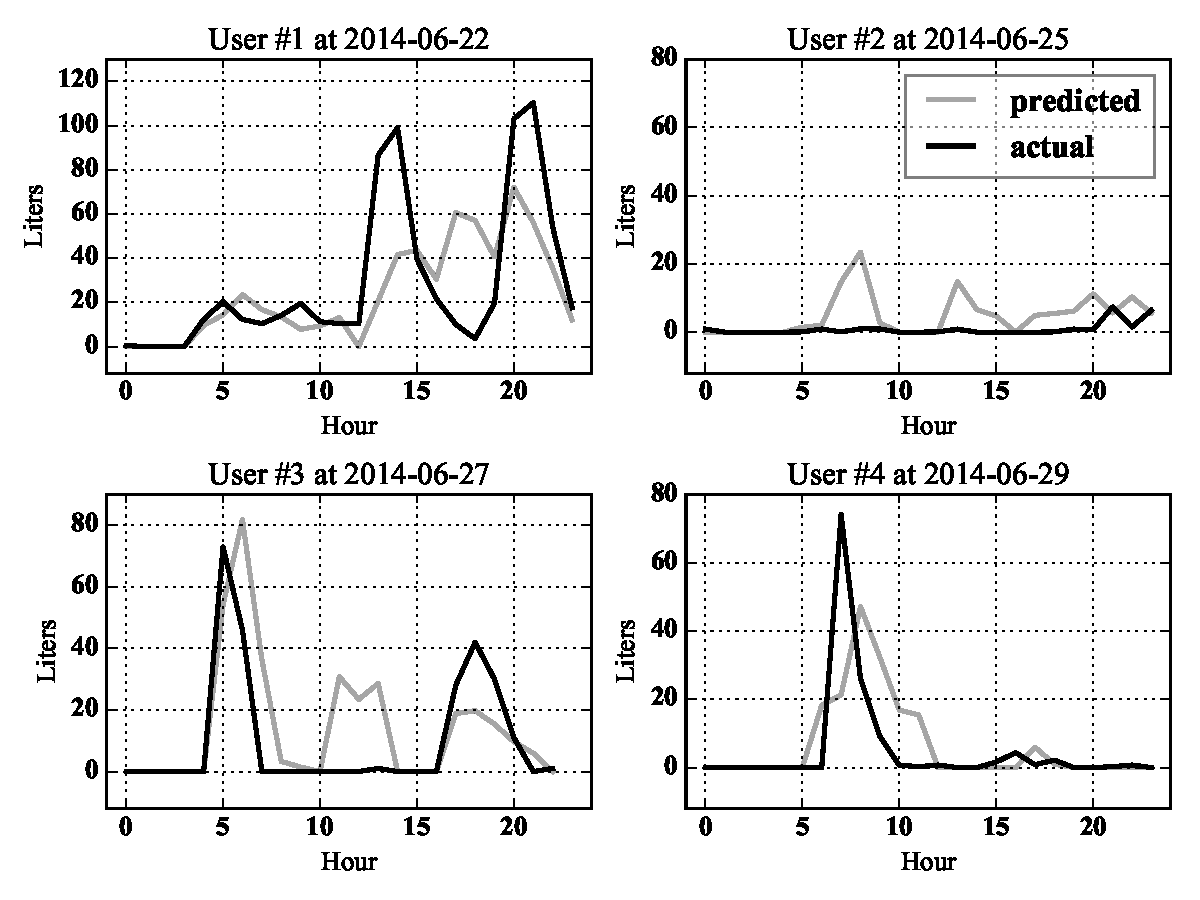
\includegraphics[width=0.75\textwidth]{figures/figure8.pdf}
	\caption{Personalised hourly water consumption prediction.}	
	\label{figure8}
\end{figure}

The results are particularly interesting if we aggregate the total predicted consumption of all users during each hour. The two upper diagrams in Figure~\ref{figure9} illustrate this case for two different days. It is apparent that our algorithms' predictions are able to properly follow the real aggregated consumption during each hour. This indicates that the negative effect of the sudden/unusual/unforeseen events is lost when we attempt to predict the total hourly water consumption of a larger number of users. The two lower diagrams present the same prediction performed by feeding our algorithms with already aggregated hourly consumption data. While the pre-aggregated dataset's predictions appear to less diverge from the actual values in certain points, the non-aggregated results are smoother and better assemble the actual overall behavior. This is due to the fact that the non-aggregated dataset also contains user-specific features and is thus able to perform predictions based on user similarity, thus, yielding more accurate predictions.

\begin{figure}[!ht]
	\centering
	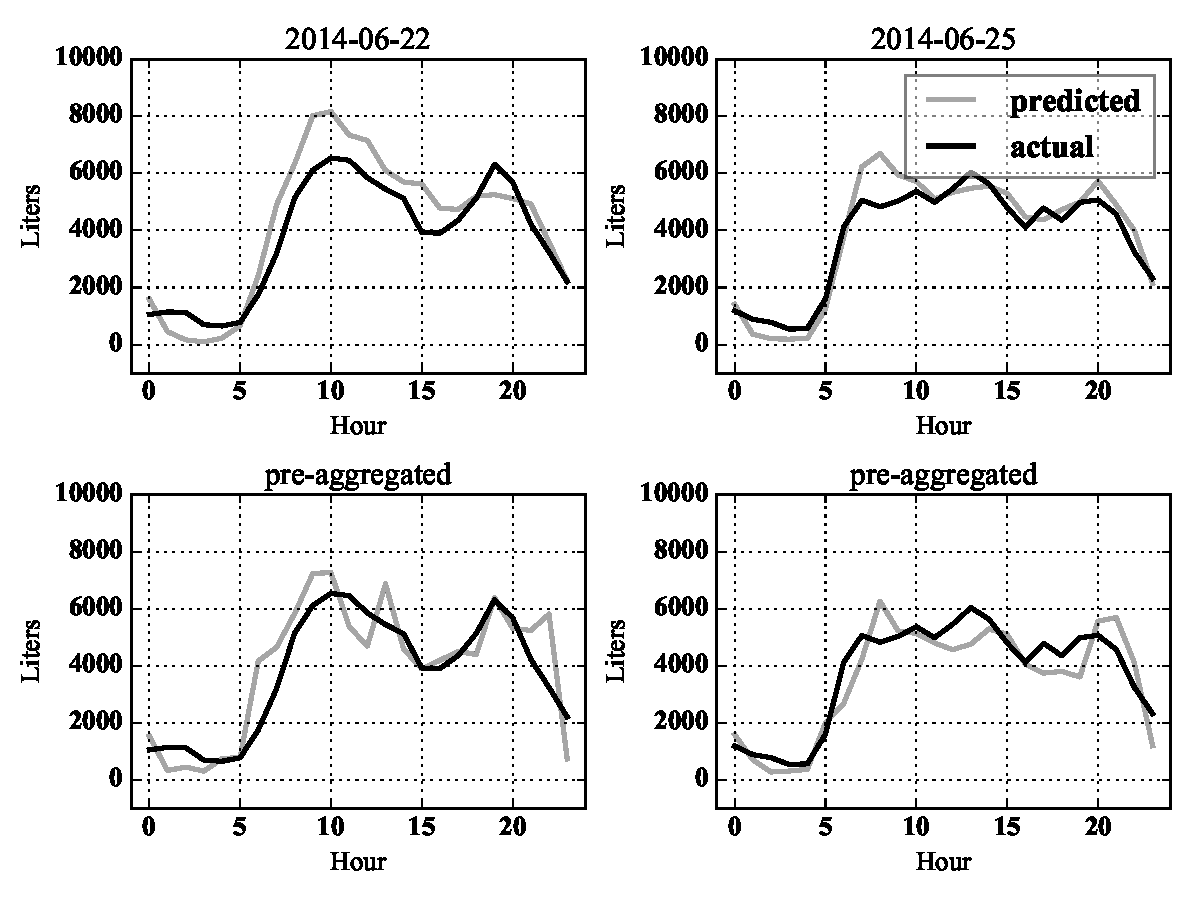
\includegraphics[width=0.75\textwidth]{figures/figure9.pdf}
	\caption{Aggregated hourly water consumption prediction.}
	\label{figure9}
\end{figure}

\subsubsection{Shower dataset}
\label{subsubsec:case_study2}
This case study exhibits the framework's potential in extracting useful knowledge from shower water consumption data, using the shower dataset. More specifically, the probabilistic classifier is used (the $z$-order curve is selected, similarly to the previous case study) in order to predict specific characteristics of a user, from shower water consumption events.

\paragraph{Feature extraction}
\label{par:feat_extr2}
As mentioned, the dataset, apart from shower water consumption related data, also included demographic information. In this case study we focused on predicting the sex, age and income of the person that generates a shower event, using classification. For the case of sex, we used the shower events for which we knew whether the person was male or female (binary classification), i.e., households with only one, or only same sex inhabitants. Consequently, each record consisted of all the smart meter measurements (shower stops, break time, shower time, average temperature, average flow rate) as features and the sex as the target variable. Due to the dataset's rather small size, the age and income prediction was also performed by binary classification, i.e., determine whether the person that generates a shower event is of age less than 35 years or not, or has income less than 3000 CHF or not. The features of each record were the same in all three cases.

\paragraph{Procedure}
\label{par:procedure2}
We ran the probabilistic classifier in order to perform binary classification of the shower events for each of the target variables. Ten-fold \textit{cross-validation} was also used in this case. The latter, similarly to the previous case, helped us determine the optimal value of $k$ parameter, which was set to 10.

\paragraph{Results}
\label{par:res2}
The results obtained by the classification are illustrated in Figure~\ref{figure10}. The classifier achieved cross-validation accuracy of 78.6\%, 64.7\% and 61.5\% for sex, age and income prediction respectively. Despite the fact that a larger dataset would generate more confident results, it is safe to conclude to that predicting the age and income of a shower-taker based solely on her showers is a non-trivial task. On the other hand, sex is easier to predict as it directly affects the actions of a person during a shower.

 \begin{figure}[!ht]
 	\centering
 	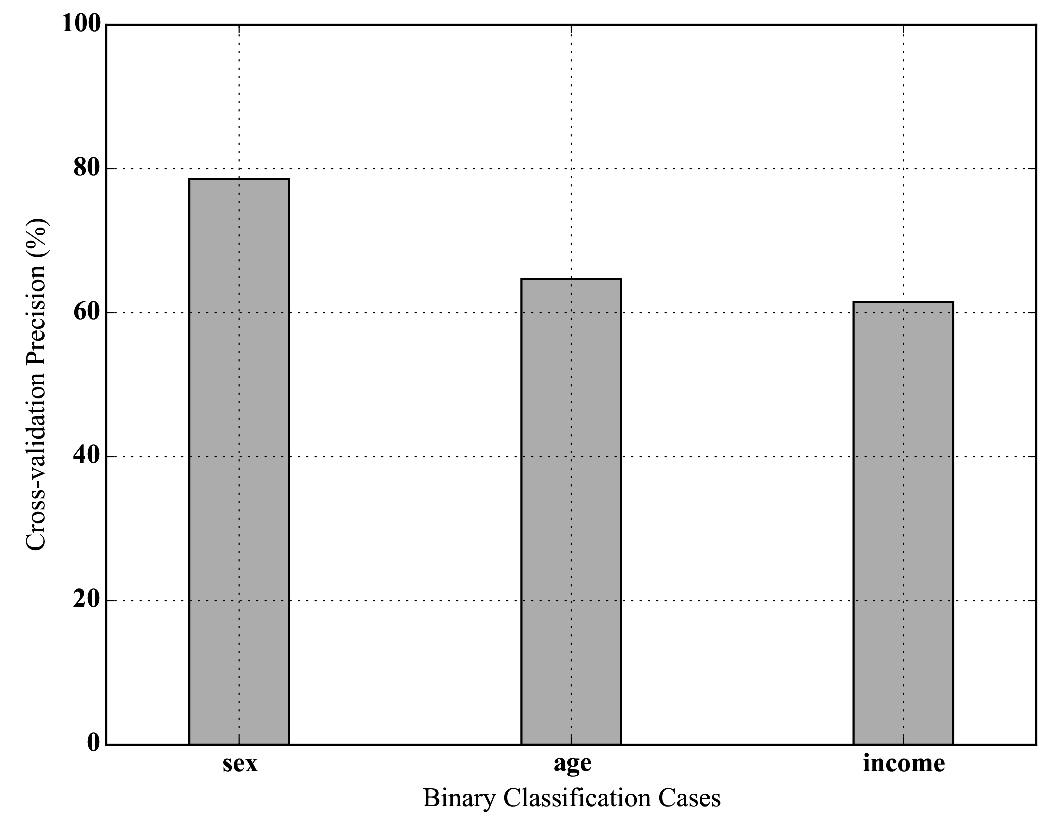
\includegraphics[width=0.75\textwidth]{figures/figure10.pdf}
 	\caption{Cross-validation accuracy for sex, age and income prediction.}	
 	\label{figure10}
 \end{figure}